\documentclass[12pt]{article} % Класса article хватит для курсовой и диплома 
\usepackage[utf8]{inputenc}
\usepackage[english,russian]{babel}
\usepackage[T2A,T1]{fontenc}
\usepackage{amsmath} % Пакет специальных символов
\usepackage{amsfonts} 
\usepackage{amssymb} % Этих пакетов хватает для набора большинства спецсимволов 
\usepackage{graphicx} % Графика
\usepackage{hyperref} % Навигация по ссылкам в документе % Продвинутое цитирование
%\usepackage{cite}
\usepackage{color} %% это для отображения цвета в коде
\usepackage{listings} %% собственно, это и есть пакет listings
\usepackage{bm}
\usepackage{caption}
\DeclareCaptionFont{white}{\color{white}} %% это сделает текст заголовка белым
%% код ниже нарисует серую рамочку вокруг заголовка кода.
\DeclareCaptionFormat{listing}{\colorbox{black}{\parbox{\textwidth}{#1#2#3}}}
\captionsetup[lstlisting]{format=listing,labelfont=white,textfont=white}
\usepackage[a4paper, top=20mm, left=30mm, right=15mm, bottom=20mm]{geometry} % Поля
\usepackage{indentfirst}
\usepackage{setspace}
\setlength{\parindent}{1.25cm} %
\renewcommand{\baselinestretch}{1}
\newcommand{\eps}{\varepsilon}
\newtheorem{Def}{Определение}
\newtheorem{Th1}{Теорема}

\title{Локальная динамика уравнения второго порядка с запаздыванием в производной}
\author{Maslenikov Igor}
\date{June 2021}

\begin{document}

\onehalfspacing
	\begin{titlepage}
		 \begin{center}
			\large
			
			\vspace{0.5cm}
			
		\vspace{0.5cm}
		
		
			\vspace{0.5cm}
			
			
			\vfill
			\vspace{0.5cm}
			
			МИНОБРНАУКИ РОССИИ
			
			
			\vspace{0.5cm}
			
		Федеральное государственное бюджетное образовательное учреждение 
		
		высшего образования
		
		\vspace{0.5cm}
		
		«Ярославский государственный университет им. П.Г. Демидова»
		
			\vspace{0.5cm}
			
			\vspace{0.5cm}
			
			\textbf{Локальная динамика уравнения второго порядка\\ с запаздыванием в производной }\\
			
			\vspace{0.5cm}

			Маслеников Игорь Николаевич

1 курс, аспирант

Кащенко Илья Сергеевич

Доктор физико-математических наук, 

заведующий кафедрой математического моделирования ЯрГУ 

			\vfill
			
			
			\bigskip
			
			
		\end{center}

	
	
	\end{titlepage}

\newpage
\section*{Abstract}

The paper consists of 16 pages. There are 3 chapters, 14 images, 11 sources in the paper.

\textbf{Characteristic quasi-polynomial, asymptotic approximation, normal form, dynamics}

The paper aims to study the model of an optoelectronic oscillator in the form of a differential integral equation with a delay:

\[
\varepsilon\frac{dx}{dt}+x+\delta\int^{t}_{t_{0}}x\left(s\right)ds=F\left(x(t-\tau)\right).
\]

\noindent We set the task of studying local dynamics in the vicinity of the equilibrium state of the equation. To do this, a characteristic equation is constructed and the position of its roots is determined. The behavior of solutions in the vicinity of the equilibrium state depending on the values of the parameters and their stability are observed. Critical values of parameters are highlighted when the equilibrium state changes its stability. An asymptotic approximation of the roots of the characteristic polynomial is obtained. An analog of the normal form is constructed. As a result of the conducted research, a differential equation was obtained, the solution of which determines the main part of the solutions of the original differential-integral equation.

\newpage 
\tableofcontents
\newpage

\addcontentsline{toc}{section}{Introduction}
\section*{Introduction}

Let's consider a model of an optoelectronic oscillator with a delay, which is an implementation of the modified Ikeda equation \cite{S1} with a time delay:




\begin{equation}
\varepsilon\frac{dx}{dt}+x+\delta\int^{t}_{t_{0}}x\left(s\right)ds=F\left(x(t-\tau)\right). \label{f:1}
\end{equation}


\noindent Replacing $x =\dot{y}$   and time normalization leads the system \eqref{f:1} to the form of the Minorsky equation \cite{P1}\eqref{f:2}:

\begin{equation}
\eps\ddot{y}+\dot{y}+\delta y= F(\dot{y}(t-1)).
\label{f:2}
\end{equation}

\noindent Here \(\tau\) --- time delay, real and positive, $\eps,\;\delta$ small parameters. The function $F$ is smooth enough, without limiting generality, we can assume that \(F(0)=0\). Thus, the equation \eqref{f:2} has a zero equilibrium state, if this is not the case, then an appropriate replacement can be made.

 The equation with the parameters  \(\varepsilon=0.005 \) and \(\delta=0.016\) was considered in the paper \cite{S1}:  numerical study was conducted, parameters and initial conditions were selected, complex quasi-periodic regimes – so-called chimeras – were constructed. Because of this, we will assume that the parameters \(\varepsilon\) and \(\delta\) are small $(0<\varepsilon\ll 1,$$0<\delta\ll1)$ and proportional to: \(k\varepsilon=\delta\), \(k>0\).

We set the task to investigate local dynamics in the vicinity of the equilibrium state. We have chosen the space  $C^1_{[-1,0]}$ as the phase space of the equation \eqref{f:2}. We fix functions $y(s)$ and $y'(s)$ on the delay length segment $s\in[-1,0]$. In the works \cite{M1}, \cite{M2}, \cite{M3}, the characteristic roots of the equation \eqref{f:2} and analogs of the normal forms of the equation \eqref{f:2} are constructed for some critical parameter values.

Note that the articles \cite{S2}, \cite{S3}, \cite{S4} consider a similar equation of an optoelectronic oscillator in which the parameter \(\delta\) is not small. In \cite{S2}, finite-dimensional and special infinite-dimensional equations are constructed, which play the role of normal forms. Asymptotic formulas for solutions for the interval $[t_0,\infty]$ are given.

\newpage

\section{Study of stability of the equilibrium state}



In \cite{M1}, the study of the location of the roots of the characteristic quasi-polynomial linearized at the zero equilibrium state of the equation \eqref{f:2} is carried out:

\begin{equation}
\eps\lambda^{2}+\lambda+k\varepsilon =\lambda\beta_1 e^{-\lambda }.
\label{f:3}
\end{equation}

\noindent The following theorems are valid.

\noindent {\bf Theorem 1.}{\sl If \(\left|\beta_1\right|<1\) and \(\eps\) is sufficiently small , all roots \eqref{f:3} have negative real parts, the zero equilibrium state is stable. If \(\left|\beta_1\right|>1\) and  \(\eps\) is sufficiently small, there are roots \eqref{f:3}having positive real parts, the zero equilibrium state is unstable.}


\noindent Proof:

Let's make a replacement in the equation \eqref{f:3} $\lambda=\dfrac{\mu}{\eps}$, then the characteristic equation \eqref{f:3} has the form:


\begin{equation}
\dfrac{\mu^2}{\eps}+\dfrac{\mu}{\eps}+k\varepsilon =\dfrac{\mu}{\eps}\beta_1 e^{-\frac{\mu}{\eps} }.
\label{f:4}
\end{equation}

Assume the opposite, that there is a root \(\mu\) with a non-negative real part, i.e. Re\(\mu\geq0\). Divide the equation \eqref{f:4} on $\dfrac{\mu}{\eps}$, this can be done because \(\mu=0\) is not a root. We get:

\begin{equation}
\mu+1+\frac{k\eps^{2}}{\mu} =\beta_1 e^{- \frac{\mu}{\eps}}.
\label{f:5}
\end{equation}

Imagine \(\mu=\alpha+i\gamma\) and evaluate the module of the right part:

\[
|\beta_1 e^{- \frac{\alpha+i\gamma}{\eps}}|=|\beta_1 ||e^{- \frac{\alpha+i\gamma}{\eps}}|\leq
|\beta_1 |e^{- \frac{\alpha+i\gamma}{\eps}}\leq|\beta_1|.
\]

\noindent Evaluate the left part:

\[
|\mu+1+\frac{k\eps^{2}}{\mu}|=
|\alpha+i\gamma+1+\frac{k\eps^{2}}{(\alpha+i\gamma)}|=|\alpha+i\gamma+1+\frac{k\eps^{2}(\alpha-i\gamma)}{(\alpha^{2}+\gamma^{2})}|=
\]

\[
=\sqrt{\left(\alpha+1+\frac{k\eps^{2}\alpha}{(\alpha^{2}+\gamma^{2})}\right)^{2} +
\left(\gamma-\frac{k\eps^{2}\gamma}{(\alpha^{2}+\gamma^{2})}\right)^{2} }.
\]

Consider the second term, it is always non-negative \(\left(\gamma-\displaystyle\frac{k\eps^{2}\gamma}{ (\alpha^{2} + \gamma^{2})}\right)^{2} \geq 0\), and since we consider the case \(\alpha\geq0\), the first term will always be at least one:

\[
\left(\alpha+1+\frac{k\eps^{2}\alpha}{(\alpha^{2}+\gamma^{2})}\right)^{2}\geq 1.
\]

It follows that for \(/\beta_1|<1\) neither on the imaginary axis nor in the right complex half-plane of the characteristic equation \eqref{f:5} there are no roots.

Consider the case $\beta_1>1$, let $\lambda=ln(\beta_1)+\mu$ substitute this value into the equation \eqref{f:3}, we get the function $F(\eps,\mu)$:

\begin{equation}
F(\eps,\mu)=\eps(ln^2\beta_1+2ln\beta_1\mu+\mu^2)+\mu+ln\beta_1+k\eps-(\mu+ln\beta_1)e^{-\mu}.
\label{f:z6}
\end{equation}


For $\eps=0$, there is a root equation \eqref{f:z6} $\mu=0$, and the function $F'_\mu(0,0)\neq 0$, hence by the implicit function theorem $\mu=o(1)$. That was what needed to be proved. The case of $\beta_1<-1$ is proved similarly.

The theorem is proved.


Thus, the case $\beta_1=\pm1$ needs additional investigation. With such values of the parameter $\beta_1$, the characteristic equation has an infinite number of roots tending to the imaginary axis.



\noindent {\bf Theorem 2.} {\sl At \(\beta_1=1+\eps^2\beta\) the roots of the characteristic equation \eqref{f:3}, located near the imaginary axis, admit an asymptotic representation of the form:}


\[
\lambda_n=\lambda_{n0}+ \varepsilon\lambda_{n1}+\varepsilon^{2}\lambda_{n2}+o(\varepsilon^{2}),\;\text{if}\;n\neq0\text {where}
\]
\[
\lambda_{n0}=2\pi ni,\;
\lambda_{n1}=-\frac{\lambda_{n0}^{2}+k}{\lambda_{n0}},
\]
\[
\lambda_{n2}=-\frac{2\lambda_{n0}\lambda_{n1}+\lambda_{n1}^2}{\lambda_{n0}}+\frac{\lambda_{n1}^2}{2}+\beta,
\]
\[
\lambda= \sqrt{\varepsilon k}i-\varepsilon\frac{k}{4}+o(\varepsilon),\;
\bar{\lambda}= -\sqrt{\varepsilon k}i-\varepsilon\frac{k}{4}+o(\varepsilon).
\]

Proof:

Assume the parameter \(\beta_1=1+\eps^2\beta\) for certainty when $\beta>0$. We select the first term of the expansion of the asymptotic series:

\[
\lambda=\lambda_{0}+o(1).
\]

\noindent is substituted into the equation \eqref{f:3} and everything that will have the order of smallness greater than \(o(1)\) group:

\[
\lambda_{0}e^{-\lambda_{0}}=\lambda_{0}+o(1).
\]

Highlighting the main part, we get:

\[
\lambda_{0} (e^{-\lambda_{0}}-1)=0.
\]

The roots of this equation are:

\[
\lambda_{0}=0\;and\;\lambda_{n0}=2\pi ni,\;n\in\mathbb{Z}\;.
\]

Note that the zero root has a multiplicity of 2. Let's refine the asymptotics for $\lambda_{n0}\neq0$ to determine the real part of each root. Imagine the decomposition of the roots of the equation \eqref{f:3} in the form of:

\[
\lambda_n=\lambda_{n0}+ \varepsilon\lambda_{n1}+\varepsilon^{2}\lambda_{n2}+о(\varepsilon^{2}),\, где\, \lambda_{n0}=2\pi n i.
\]

Substitute the decomposition of the roots into the equation \eqref{f:3}, we get:

\[
\eps\left(\lambda_{n0}+ \varepsilon\lambda_{n1}\right)^{2}+\lambda_{n0}+ \varepsilon\lambda_{n1}+\varepsilon^{2}\lambda_{n2}+k\varepsilon+ o(\varepsilon^{2})= 
\]
\[
= (1+\ eps^2\beta)\left(\lambda_{n0}+ \varepsilon\lambda_{n1}+\varepsilon^{2}\lambda_{n2}\right) e^{-\left(\lambda_{n0}+\varepsilon\lambda_{n1}+\varepsilon^{2}\lambda_{n2}+o(\varepsilon^{2 }\right) }.
\]

Since \(\varepsilon\lambda_{n1}+\varepsilon^{2}\lambda_{n2}\) is small, we decompose the exponent into a Taylor series:

\begin{equation}
\begin{array}{cc}
\varepsilon\left(\lambda_{n0}^{2}+\varepsilon\lambda_{n0}\lambda_{n1}\right)+\lambda_{n0}+\varepsilon\lambda_{n1}+\varepsilon^{2}\lambda_{n2}+k\varepsilon+ o(\varepsilon^{2})=\\
=(1+\eps^2\beta)\left(\lambda_{n0}+ \varepsilon\lambda_{n1}+\varepsilon^{2}\lambda_{n2}\right)
\left(1-\varepsilon\lambda_{n1}-\varepsilon^{2}\lambda_{n2}+\frac{\varepsilon^{2}}{2}\lambda_{n1}^{2}+ o(\varepsilon^{2})\right).
\end{array}
\label{f:6}
\end{equation}

Let's open the brackets and equate the coefficients for the same degrees of a small parameter.

When \(\varepsilon^{0}\) we have the correct identity:

\[
\lambda_{n0}=\lambda_{n0},\,
\lambda_{n0}=2\pi n i.
\]

With \(\varepsilon^{1}\) we get:

\begin{equation}
\begin{array}{cc}
\lambda_{n0}^{2}+\lambda_{n1}+k=
\lambda_{n1}-\lambda_{n0}\lambda_{n1},\;\text{at}\;n\neq0,\\
\lambda_{n1}=\displaystyle\frac{\left(-4\pi^{2}n^{2}+k\right)i}{2\pi n},\;\text{at}\;n\neq0.
\end{array}
\label{f:7}
\end{equation}

With \(\varepsilon^{2}\) we get:

\begin{equation}
\begin{array}{cc}
2\lambda_{n0}\lambda_{n1}+\lambda_{n2}=
\lambda_{n2}-\lambda_{n1}^{2}-\lambda_{n0}\left(\lambda_{n2}-\displaystyle\frac{\lambda_{n1}^{2}}{2}\right)\\
\lambda_{n2}=-\displaystyle\frac{2\lambda_{n0}\lambda_{n1}+\lambda_{n1}^2}{\lambda_{n0}}+\displaystyle\frac{\lambda_{n1}^2}{2}+\beta,\\
\lambda_{n2}=\left(4\pi n-\displaystyle\frac{k}{\pi n}-\displaystyle\frac{4\pi^2n^2-2k+\displaystyle\frac{k^2}{4\pi^2n^2}}{2\pi n}\right)i-\\
-\displaystyle\frac{1}{2}\left(4\pi^2n^2-2k+\displaystyle\frac{k^2}{4\pi^2n^2}\right)+\beta,\;\text{при}\;n\neq0.
\end{array}
\label{f:8}
\end{equation}


Let's do the same for \(\beta=1+\eps^2\beta_1\) and \(n=0\). Imagine the decomposition of the roots of the equation \eqref{f:3} in the form of:

\[
\lambda= \sqrt{\varepsilon}\lambda_{1}+\varepsilon\lambda_{2}+\varepsilon^{\frac{3}{2}}\lambda_{3}+o(\varepsilon^{\frac{3}{2}}).
\]

\noindent Similarly, we perform the same actions, as a result we get:

\[
\lambda_{1}=\pm \sqrt{ k}i,\;\;\lambda_{2}=\frac{-k}{4}.
\]

The theorem is proved.

The trajectory of the roots of the characteristic equation \eqref{f:3} at $\beta_1=1+\eps^2\beta$, $\eps\to 0$ and a fixed value of the parameters $k=2$, $\beta=1$ is shown in Fig. 1 :

\begin{figure}[h!]
\center{ 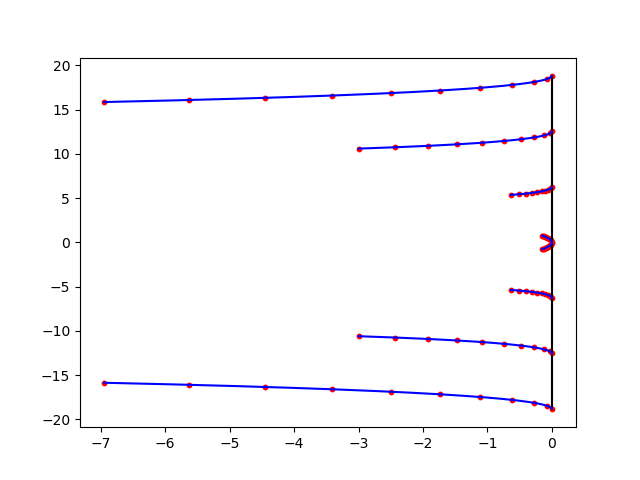
\includegraphics[scale=0.5]{+1}}
\caption{The trajectory of the roots at $\beta_1=1+\eps^2$, $\eps\to 0$.}%picture caption
\label{fig:11}
\end{figure}
Similar constructions can be carried out with \(\beta_1=-(1+\eps^2\beta)\).

\noindent {\bf Theorem 3.} {\sl At \(\beta_1=-(1+\eps^2\beta)\)the roots of the characteristic equation \eqref{f:3} $\lambda$ and $\lambda_n$, located near the imaginary axis, admit an asymptotic representation of the form:}
\[
\lambda_n=\lambda_{n0}+ \varepsilon\lambda_{n1}+\varepsilon^{2}\lambda_{n2}+o(\varepsilon^{2}),\,\text{when }n\neq0\text{, where} 
\]
\[
\lambda_{n0}=\pi (2n+1)i,\;
\lambda_{n1}=-\frac{\lambda_{n0}^{2}+k}{\lambda_{n0}},
\]
\[
\lambda_{n2}=-\frac{2\lambda_{n0}\lambda_{n1}+\lambda_{n1}^2}{\lambda_{n0}}+\frac{\lambda_{n1}^2}{2}+\beta,
\]
\[
\lambda= \frac{-\varepsilon k}{2}+o(\varepsilon) .
\]


The trajectory of the roots of the characteristic equation \eqref{f:3} at $\beta_1=-(1+\eps^2\beta)$, $\eps\to 0$ and a fixed value of the parameters $k=2$, $\beta=1$ is shown in Fig. 2 :

\begin{figure}[h!]
\center{ 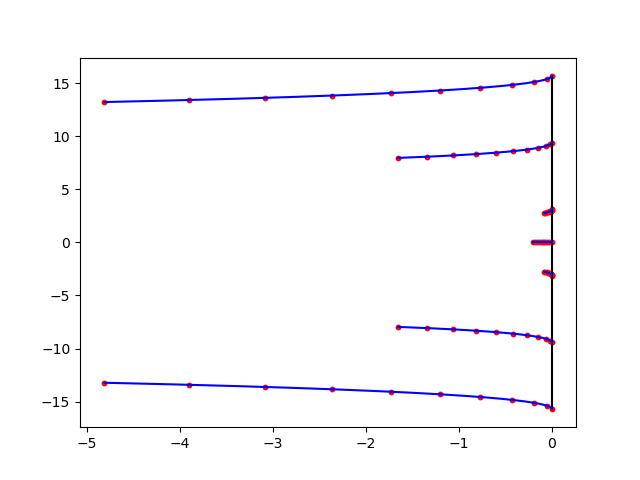
\includegraphics[scale=0.5]{-1}}
\caption{The trajectory of the roots at $\beta_1=-(1+\eps^2)$, $\eps\to 0$.}%figure caption
\label{fig:12}
\end{figure}

Thus, at $|\beta_1|$ close to 1, the characteristic equation has a countable number of roots, the real part of which tends to zero at $\eps\rightarrow 0$.

Next, we study the behavior of solutions of the equation \eqref{f:2} in the neighborhood of zero at $|\beta_1|$ close to 1 and small $\eps$.

\newpage

\section{Construction of the normal form of the equation}

Let's study the changes in the behavior of solutions of the equation \eqref{f:2} when passing $\beta_1$ through $\pm1$. Decompose in the equation \eqref{f:2} the function \(F\) in the Taylor series in the neighborhood of zero:
\begin{equation}
\eps\ddot{y}+\dot{y}+k\eps y=\beta_1\dot{y}(t-1)+\beta_2(\dot{y}(t-1))^2+\beta_3(\dot{y}(t-1))^3+\ldots,
\label{f:9}
\end{equation}

\noindent where \(\beta_2,\beta_3\) are some constants, and $\beta_1$ is close to $\pm1$: $\beta_1=\pm(1+\eps^2\beta)$.

\subsection{Constructing a normal form for $\beta_1=-(1+\eps^2\beta)$}

Consider the problem of constructing a normal form for the equation \eqref{f:9} with the parameter \(\beta_1=-(1+\eps^2\beta)\). With such a \(\beta_1\), the characteristic equation has an infinite number of roots tending to the imaginary axis, thus a critical case of infinite dimension is realized. Let's represent the function \(y\) as an asymptotic series:

\begin{equation}
y=\eps V(\tau,t)+\eps W(\tau)+\eps^2U_1(\tau,t)+\eps^3U_2(\tau,t)+\ldots,
\label{f:10}
\end{equation}

\noindent where \(U_1\), \(U_2\) are periodic with period 1: \(U_1(\tau,t)\equiv U_1(\tau,t+1)\), \(U_2(\tau,t)\equiv U_2(\tau,t+1)\). The function \(W\) is such that the average value of \(\beta_2\dot{V}^2-kW\) is 0, that is:
\[
W(\tau)=\frac{\beta_2}{k}\int\limits_0^1\left(\displaystyle\frac{\partial V}{\partial t}\right)^2(\tau,t)dt.
\]
\noindent Function \(V(\tau,t)\) is represented as a Fourier series:

\[
V(\tau,t)=\sum\limits_{\substack{ -\infty }}^\infty e^{am(\lambda_{n, 0}+ \varepsilon\lambda_{n-1}+\varepsilon^{2}\lambda_{n-2}+\ldots)t}V_n(\tau),\,\text{where}\,
\tau=\eps^2t.
\]

\noindent Values \(\lambda_{n 0}\), \(\lambda_{n 1}\), \(\lambda_{n 2}\) are determined from the asymptotic approximation of the roots of the equation \eqref{f:3} (see Theorem 3).

Substitute \eqref{f:10} into the equations \eqref{f:9}, we will equate the coefficients for the same degrees of the small parameter \(\eps\).

When \(\varepsilon \) we get the correct identity:

\[
\lambda_{n0}V_n(\tau)e^{\xi_nt}=\lambda_{n0}V_n(\tau)e^{\xi_nt}.
\]

When \(\varepsilon^2\) we get:

\begin{equation}
\begin{array}{cc}
\sum\limits_{\substack{ -\infty }}^\infty\lambda_{n0}^2V_n(\tau)e^{\xi_nt}+\sum\limits_{\substack{ -\infty }}^\infty\lambda_{n1}V_n(\tau)e^{\xi_nt}+\dot U_1+\sum\limits_{\substack{ -\infty }}^\infty kV_n(\tau)e^{\xi_nt}+\\ +kW(\tau)=\sum\limits_{\substack{ -\infty }}^\infty (-1)(-\lambda_{n1}V_n(\tau)+\lambda_{n1}\lambda_{n0}V_n(\tau))e^{\xi_nt}
-\dot{U}_1(t-1)+\beta_2\dot{V}^2.
\end{array}
\label{f:f22}
\end{equation}


\noindent  \(\dot{U}_1\)  is defined from equation  \eqref{f:f22} after reductionin the case under consideration:

\[
\dot{U}_1=\frac{1}{2}(\beta_2\dot{V}^2-kW(\tau)).
\]

\noindent \(U_1\) is in the form:
\[
U_1=\frac{1}{2}\int\limits_0^r\beta_2\dot{V}^2(s,\tau)-W(\tau)ds.
\]

Note that $U_1$ is periodic, because the average value of the integrand is zero.

When \(\varepsilon^3\) we get:

\begin{equation}
\begin{array}{cc}
\sum\limits_{\substack{ -\infty }}^\infty e^{\xi_nt}2\lambda_{n0}\lambda_{n1}V_n(\tau)+\ddot{U_1}+\sum\limits_{\substack{ -\infty }}^\infty(\lambda_{n2}V_n(\tau)+V_n'(\tau))e^{\xi_nt}+\dot{U_2}+\\
+kU_1+W'(\tau)=\sum\limits_{\substack{ -\infty }}^\infty(-1)e^{\xi_nt}((-1)(\lambda_{n2}V_n(\tau)-\lambda_{n0}V_n'(\tau)+V_n'(\tau))+\\
+\lambda_{n1}^2V_n(\tau)+(-\lambda_{n2}+\displaystyle\frac{1}{2}\lambda_{n1}^2)\lambda_{n0}V_n(\tau))-(\dot{U}_2(t-1)+W'(\tau))+\\
+\sum\limits_{\substack{ -\infty }}^\infty\lambda_{n0}\beta V_n(\tau)e^{\xi_nt}+\dot{U_1}(t-1)+\beta_2\sum\limits_{\substack{ -\infty }}^\infty\varphi_{2n}(V)e^{(\pi(2n+1)i+o(\eps))t}+\\
+\beta_2\sum\limits_{\substack{ -\infty }}^\infty f_{2n}(V)e^{(\pi2ni+o(\eps))t}+\beta_3\sum\limits_{\substack{ -\infty }}^\infty\varphi_{3n}(V)e^{(\pi(2n+1)i+o(\eps))t},
\end{array}
\label{f:f23}
\end{equation}

\noindent where \(\varphi_{2n}(V)\) Fourier series coefficients for the function:
\[
-2\dot{U}_1(t-1)\sum\limits_{\substack{ -\infty }}^\infty\pi(2n+1)i V_n(\tau)e^{\xi_nt};
\]

\noindent \(\varphi_{3n}(V)\) Fourier series coefficients for the function:
\[
-\left(\sum\limits_{\substack{ -\infty }}^\infty\pi(2n+1)i V_n(\tau)\right)^3;
\]

\noindent\(f_{2n}(V)\) coefficients of the Fourier series for the function:
\[
-2\sum\limits_{\substack{ -\infty }}^\infty\lambda_{n0} V_n(\tau)e^{\xi_nt}\cdot\sum\limits_{\substack{ -\infty }}^\infty\lambda_{m0}\lambda_{m1}V_m(\tau) e^{\xi_mt}.
\]

Equation \eqref{f:f23} is simplified to the form:

\begin{equation}
\begin{array}{cc}
\ddot{U_1}+2\dot{U}_2+kU_1+2W'(\tau)-\beta_2\sum\limits_{\substack{ -\infty }}^\infty f_{2n}(V)e^{(\pi2ni+o(\eps))t}=\\
\sum\limits_{\substack{ -\infty }}^\infty(-\lambda_{n0}V_n'(\tau)+\displaystyle\frac{1}{2}\lambda_{n1}^2\lambda_{n0}V_n(\tau)+\lambda_{n0}\beta V_n(\tau)+\\
+\beta_2\varphi_{2n}(V)+\beta_3\varphi_{3n}(V))e^{(\pi(2n+1)i+o(\eps))t}.
\end{array}
\label{f:f24}
\end{equation}

In the equation \eqref{f:f24} the left part is periodic and the right part is antiperiodic, equality is possible if and only if the left and right parts are equal to 0.

\(\dot{U_2}\) is defined as:
\[
\dot{U}_2=\frac{1}{2}(\beta_2\sum\limits_{\substack{ -\infty }}^\infty f_{2n}(V)e^{(\pi2ni+o(\eps))t}-\ddot{U_1}-kU_1-2W'(\tau)).
\]
Consider the antiperiodic part of the equation \eqref{f:f24} and decompose it into the corresponding degrees \(e^{\xi_nt}\):
\begin{equation}
\begin{array}{cc}
\lambda_{n0}V_n'(\tau)=\displaystyle\frac{1}{2}\lambda_{n1}^2\lambda_{n0}V_n(\tau)+\lambda_{n0}\beta V_n(\tau)+\beta_2\varphi_{2n}(V)+\beta_3\varphi_{3n}(V).
\end{array}
\label{f:f25}
\end{equation}

Substitute the values \(\lambda_{n1}\) and \(\lambda_{n0}\) into the equation \eqref{f:f25}:
\begin{equation}
\begin{array}{cc}
V_n'(\tau)=-\displaystyle\frac{1}{2}\left(\pi^2 (2n+1)^2-2k+\frac{k^2}{\pi^2(2n+1)^2}\right)V_n(\tau)+\\
+\beta V_n(\tau)+\displaystyle\frac{\beta_2}{\pi (2n+1)i}\varphi_{2n}(V)+\displaystyle\frac{\beta_3}{\pi (2n+1)i}\varphi_{3n}(V).
\end{array}
\label{f:f26}
\end{equation}



In the works \cite{M2}, \cite{M3} it was shown that the equation \eqref{f:9} in the case under consideration is reduced to a partial differential equation \eqref{f:11} with boundary conditions:

\begin{equation}
\displaystyle\frac{\partial V}{\partial \tau}=\frac{1}{2}\frac{\partial^2 V}{\partial^2 t}+kV-\frac{k^2}{2}J^2(V)+\beta V+ \beta_2J\left(U_1\frac{\partial V}{\partial t}\right)+\beta_3J\left(\left(\frac{\partial V}{\partial t}\right)^3\right),
\label{f:11}
\end{equation}

\begin{equation}
\begin{array}{cc}
\int\limits_0^1V(\tau,t)dt=0,\;V(\tau,t) \equiv -V(\tau,t+1).
\end{array}
\label{f:12}
\end{equation}

\noindent $J(V)$ denotes the primitive function $V$ with zero mean:

\[
J^2(V)=J(J(V)),\,(J(V))'_t\equiv V.
\]

The following theorem is true \cite{M2}, \cite{M3}:

\noindent {\bf Theorem 4.} {\sl Let \(V_*\) be a bounded solution \eqref{f:11} with boundary conditions \eqref{f:12}, with \(V_*=\sum\limits_{\substack{ -\infty}}^\infty e^{\pi(2n+1)i t}V_n(\tau)\), then

\[
y(t)=\eps\sum\limits_{\substack{ -\infty }}^\infty e^{iIm(\lambda_{n0}+ \varepsilon\lambda_{n1}+\varepsilon^{2}\lambda_{n2}+\ldots) t}V_n(\tau)+\eps \dfrac{\beta_2}{k}\int\limits_0^1\dot{V}^2(t,\tau)dt,
\]
\noindent where $\tau=\eps^2 t$ is a slow time, the values \(\lambda_{n0}\), \(\lambda_{n1}\), \(\lambda_{n2}\) are defined in Theorem 3, is asymptotic in the residual with accuracy $O(\eps^3)$ uniformly over \(t\geq 0\) solution \eqref{f:9}}.

Thus, the problem \eqref{f:11}, \eqref{f:12} is an analogue of the normal form for the equation \eqref{f:9}, with a critical value of the parameter $\beta_1=-(1+\eps^2\beta)$. Note that the coefficients of the boundary value problem do not depend on the parameter $\eps$.










\subsection{Constructing a normal form with $\beta_1=1+\eps^2\beta$ }

Consider the equation \eqref{f:2} with the parameter $\beta_1=1+\eps^2\beta$, then the equation \eqref{f:2} has the form \eqref{f:19}:

\begin{equation}
\eps y''+y'+k\eps y=\beta_1y'(t-1)+\beta_2y'^2(t-1)+\beta_3y'^3(t-1)\cdots.
\label{f:19}
\end{equation}

Let's imagine the function \(y\) as a series:

\begin{equation}
y=\eps^{\frac{1}{4}}(W(\tau)e^{is}+C.C.)+\eps^2 V(\eta,t)+U(\eta,\tau,s,t)+\ldots,
\label{f:20}
\end{equation}

\noindent where $\tau=\eps t,\;\eta=\eps^2t,\;s=\sqrt{\eps k}t$slow times, $U(\tau,\eta,s,t)=U(\tau,\eta,s,t-1)$ is a periodic function of $t$. The function $V(\eta,t)$ has the form:

\begin{equation*}
V=\sum_{n\neq0}V_n(\tau)e^{iIm(\lambda_{n0}+ \varepsilon\lambda_{n1}+\varepsilon^{2}\lambda_{n2}+\ldots)t}=\sum_{n\neq0}V_n(\tau)e^{\xi_nt}.
\end{equation*}

\noindent Values \(\lambda_{n0}\), \(\lambda_{n1}\), \(\lambda_{n2}\) are determined from the asymptotic approximation of the roots of the equation \eqref{f:3} (see Theorem 2).

The function $U(\eta,\tau,s,t)$ is representable as a sum of series:

\begin{equation*} 
\begin{array}{cc}
U(\eta,\tau,s,t)=\eps^{\frac{1}{2}}\sum\limits_{n=0}^\infty \eps^{\frac{n}{4}}H_n(\tau,s)
+\eps^{\frac{9}{4}}(\sum\limits_{n=0}^\infty \eps^{\frac{n}{4}}D_n(\eta,\tau,s,t)) +\eps^{3}(\sum\limits_{n=0}^\infty \eps^{\frac{n}{4}}R_n(\eta)).
\end{array}
\end{equation*}

Substitute \eqref{f:20} into the equation \eqref{f:19}, open the brackets, equate the coefficients for the same degrees of the small parameter \(\eps\). Functions from $U(\tau,\eta,s,t)$ will be sequentially defined from $W(\tau)e^{is}+C.C.$ and $V(\eta,t)$.

For $\eps^{\frac{3}{2}}$, the function $H_0$ is defined:

\begin{equation*}
\begin{array}{c}
0=kH_0(\tau,s)+kH_0^{ss}(\tau,s)+
\beta_2k(e^{2is}W^2(\tau)+e^{-2is}\overline{W}^2(\tau)-2W(\tau)\overline{W}(\tau)),
\end{array}
\end{equation*}


\begin{equation*}
\begin{array}{c}
H_0(\tau,s)=
\dfrac{\beta_2}{3}(2ie^{2is}W^2(\tau)+e^{-2is}\overline{W}^2(\tau))+2\beta_2W(\tau)\overline{W}(\tau).
\end{array}
\end{equation*}

The function $W$ is defined at $\eps^{\frac{7}{4}}$:


\begin{equation*}
\begin{array}{c}
0=kH_1(\tau,s)+kH_1^{ss}(\tau,s)+\\
\dfrac{1}{2}ie^{is}k^{\frac{3}{2}}W(\tau)-\eps\beta ie^{is}\sqrt{k}W(\tau)+2ie^{is}\sqrt{k}W^{\tau}(\tau)-\\
-(\dfrac{1}{2}ie^{-is}k^{\frac{3}{2}}\overline{W}(\tau)-\eps\beta ie^{-is}\sqrt{k}\overline{W}(\tau)+2ie^{-is}\sqrt{k}\overline{W}^{\tau}(\tau))+\\
2\dfrac{\beta_2^2}{3}(2i\sqrt{k}e^{2is}W^2(\tau)-2i\sqrt{k}e^{-2is}\overline{W}^2(\tau))(-i\sqrt{k}e^{is}W(\tau)+i\sqrt{k}e^{-is}\overline{W}(\tau)).
\end{array}
\end{equation*}

Equate the coefficients for the same $e^{is}$ and $e^{-is}$:

\begin{equation*}
\begin{array}{c}
2ie^{is}\sqrt{k}W^{\tau}(\tau)=-\dfrac{1}{2}ie^{is}k^{\frac{3}{2}}W(\tau)+\eps\beta ie^{is}\sqrt{k}W(\tau)+\\
+4\dfrac{\beta_2^2}{3}ke^{is}W^2(\tau)\overline{W}(\tau)+3i\beta_3\eps^{\frac{1}{2}}k^{\frac{3}{2}}e^{is}W^2(\tau)\overline{W}(\tau),\\
2ie^{-is}\sqrt{k}\overline{W}^{\tau}(\tau)=-\dfrac{1}{2}ie^{-is}k^{\frac{3}{2}}\overline{W}(\tau)+\eps\beta ie^{-is}\sqrt{k}\overline{W}(\tau)-\\
-4\dfrac{\beta_2^2}{3}ke^{-is}W(\tau)\overline{W}^2(\tau)-3i\beta_3\eps^{\frac{1}{2}}k^{\frac{3}{2}}e^{-is}W(\tau)\overline{W}^2(\tau),
\end{array}
\end{equation*}


\begin{equation}
\begin{array}{c}
W^\tau(\tau)=(\dfrac{\eps\beta}{2}-\dfrac{k}{4})W(\tau)-\dfrac{2}{3}\beta_2^2\sqrt{k}iW^2(\tau)\overline{W}(\tau)+\dfrac{3}{2}\beta_3\eps^{\frac{1}{2}}kW^2(\tau)\overline{W}(\tau),\\
\overline{W}^\tau(\tau)=(\dfrac{\eps\beta}{2}-\dfrac{k}{4})\overline{W}(\tau)+ \dfrac{2}{3}\beta_2^2\sqrt{k}iW(\tau)\overline{W}^2(\tau)-\dfrac{3}{2}\beta_3\eps^{\frac{1}{2}}kW(\tau)\overline{W}^2(\tau).
\end{array}
\label{f:y22}
\end{equation}

Note that for $\eps\beta<\dfrac{k}{2}$ the solution of the equation \eqref{f:y22} tends to zero.


The function $V_n$ is defined from the expression:
\begin{equation*} 
\begin{array}{c}
\sum\limits_{n\neq0}V_n^{\eta}(\eta)e^{\xi_nt}\lambda_{n0}=\sum\limits_{n\neq0}V_n(\eta)e^{\xi_nt}\dfrac{1}{2}\lambda_{n1}^2\lambda_{n0}+\beta\sum\limits_{n\neq0}V_n(\eta)e^{\xi_nt}\lambda_{n0}+\\
+\beta_3(\sum\limits_{n\neq0}V_n(\eta)e^{\xi_nt}\lambda_{n0})^3.
\end{array}
\end{equation*}


The equation \eqref{f:19} in the considered case is reduced to considering a partial differential equation \eqref{f:21} with boundary conditions \eqref{f:22}:
\begin{equation}
\displaystyle\frac{\partial V}{\partial \eta}=\frac{1}{2}\frac{\partial^2 V}{\partial^2 t}+kV-\frac{k^2}{2}J^2(V)+\beta V+ \beta_3J\left(\left(\frac{\partial V}{\partial t}\right)^3\right),
\label{f:21}
\end{equation}
\begin{equation}
\begin{array}{cc}
\int\limits_0^1V(\eta,t)dt=0,\;
V(\eta,t) \equiv V(\eta,t+1).
\end{array}
\label{f:22}
\end{equation}
\noindent $J(V)$ denotes the primitive function $V$ with zero mean:
\[
J^2(V)=J(J(V)),\,(J(V))'_t\equiv V.
\]






\noindent {\bf Theorem 5.} {\sl Let $\eps\beta<\dfrac{k}{2}$, then \(V_*(\eta,t)\) is a bounded solution with its derivatives, \eqref{f:21} with boundary conditions \eqref{f:22}, and \(V_*(\eta,t)=\sum\limits_{\substack{ -\infty}}^\infty e^ {2\pi n i t}V_n(\eta)\), then

\[
y(t)=\eps^2\sum\limits_{\substack{ -\infty }}^\infty e^{iIm(\lambda_{n0}+ \varepsilon\lambda_{n1}+\varepsilon^{2}\lambda_{n2}+\ldots) t}V_n(\eta),
\]

\noindent where $\eta=\eps^2 t$, $\tau=\eps t$, $s=\sqrt{\eps k}t$, is asymptotic in the residual with an accuracy of $O(\eps^3)$ uniformly over \(t\geq 0\) solution \eqref{f:19}}.

Note that if $\eps\beta$ is a lot, then the solution of the original equation is affected by the solution of the equation \eqref{f:y22}, the amplitude and the oscillation period change.







\newpage

\section{Numerical calculation results}

Using numerical calculation, we show how the dynamics of solutions of the equation \eqref{f:9} changes when the parameters change.

Consider as an example $F(\dot{y}(t-1))=\beta_1\sin(\dot{y}(t-1))$, and construct graphs of solutions to the equation \eqref{f:9}. Decompose the function $F$ into a Taylor series:
\[
F(\dot{y}(t-1))=\pm(1+\eps^2\beta)\dot{y}(t-1)\pm\dfrac{1}{6}(1+\eps^2\beta)\dot{y}^{3}(t-1).
\]
Thus, the task \eqref{f:9} has the form:
\begin{equation}
\eps\ddot{y}+\dot{y}+k\eps y=\pm(1+\eps^2\beta)\dot{y}(t-1)\pm\displaystyle\frac{1}{6}(1+\eps^2\beta)(\dot{y}(t-1))^3+\ldots.
\label{f:23}
\end{equation}
With the parameter $|\beta_1|<1$, the trajectory of the solution of the equation \eqref{f:23} tends to zero. The zero state of equilibrium is stable.

With the parameter $\beta_1<-1$, the trajectory of the solution of the equation \eqref{f:23} tends to the oscillatory mode. The zero state of equilibrium becomes unstable. Figure 3 shows graphs of steady-state modes at $\beta_1$ close to $-1$: $\beta_1=-(1+\eps^2\beta)$.

\begin{figure}[h!]
\begin{minipage}[h]{0.49\linewidth}
\center{a)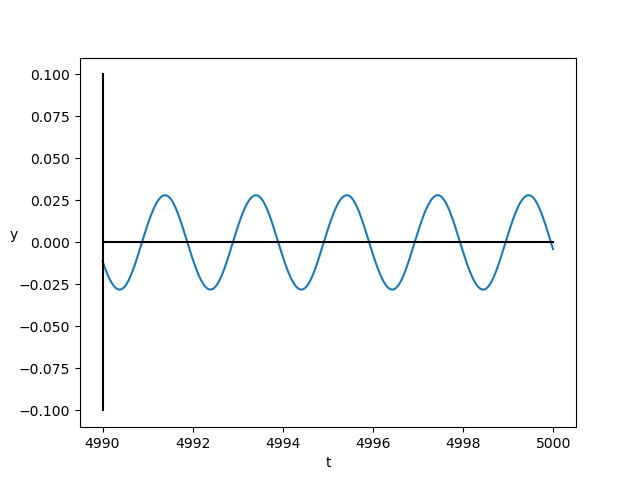
\includegraphics[scale=0.4]{min1beta=1_00125eps=0_01_4990-5000}}
\end{minipage}
\begin{minipage}[h]{0.49\linewidth}
\center{b)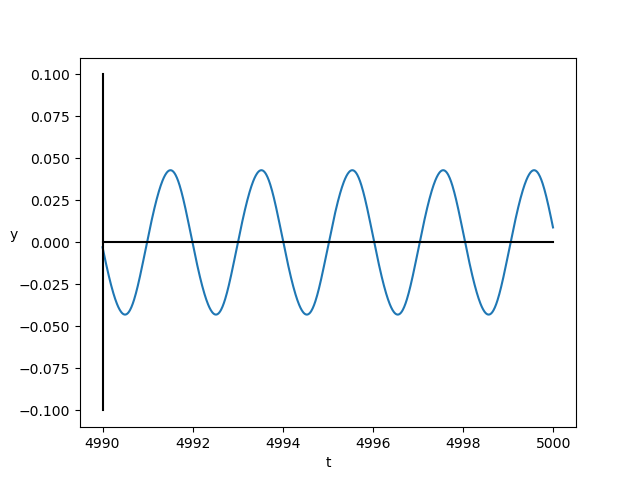
\includegraphics[scale=0.4]{min1beta=1_0025eps=0_01_4990-5000}}
\end{minipage}
\begin{minipage}[h]{0.49\linewidth}
\center{in)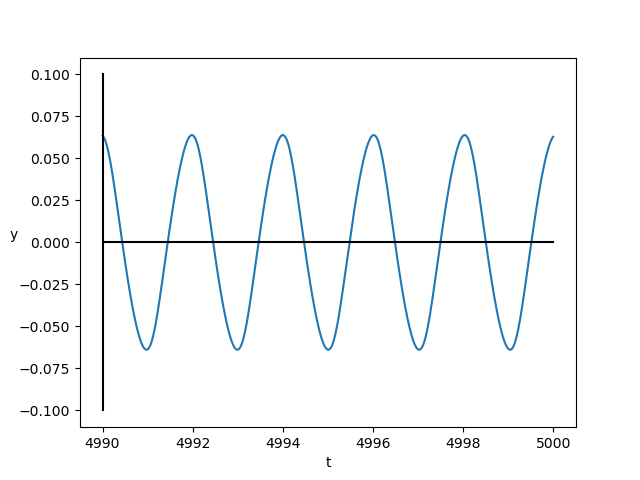
\includegraphics[scale=0.4]{min1beta=1_005eps=0_01_4990-5000}}
\end{minipage}
\begin{minipage}[h]{0.49\linewidth}
\center{d)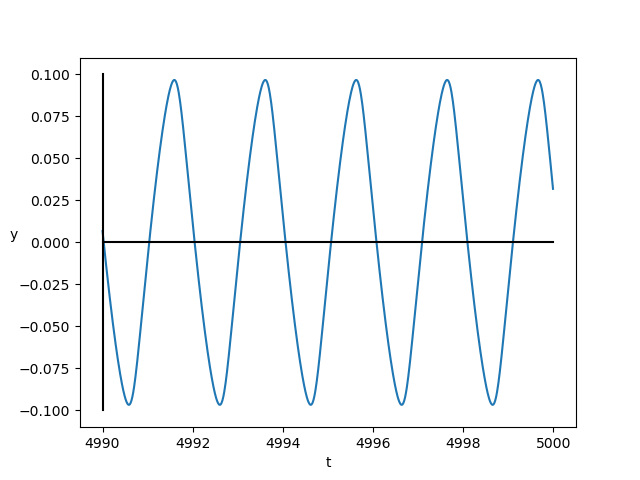
\includegraphics[scale=0.4]{min1beta=1_01eps=0_01_4990-5000}}
\end{minipage}
\caption{Graph of the solution of the equation \eqref{f:23} for $\beta_1=-(1+\eps^2\beta),\;\eps=0.01,\; k=2, $a) $\beta=12.5$, b) $\beta=25$, c) $\beta=50$, d) $\beta=100$.}%picture caption
\label{fig:4}
\end{figure}

Similarly, Figure 4 shows graphs of steady-state modes at $\beta_1$ close to 1: $\beta_1=1+\eps^2\beta$.

\begin{figure}[h!]
\begin{minipage}[h]{0.49\linewidth}
\center{a)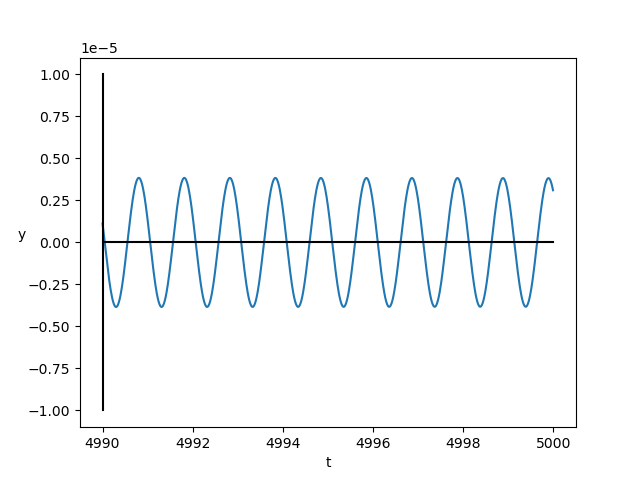
\includegraphics[scale=0.4]{plus1beta=1_00125eps=0_01_4990-5000}}
\end{minipage}
\begin{minipage}[h]{0.49\linewidth}
\center{b)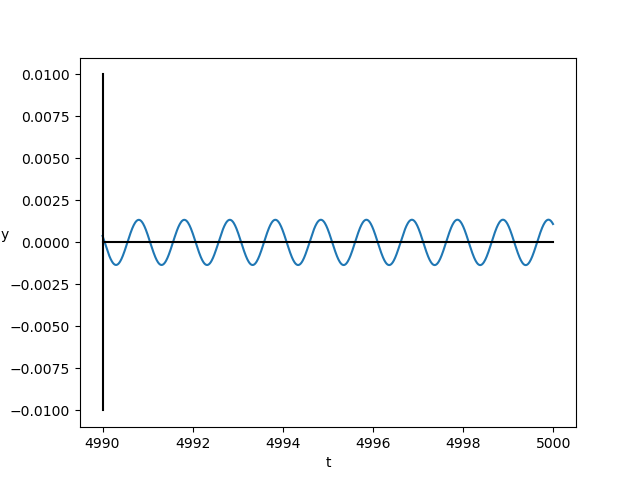
\includegraphics[scale=0.4]{plus1beta=1_0025eps=0_01_4990-5000}}
\end{minipage}
\begin{minipage}[h]{0.49\linewidth}
\center{in)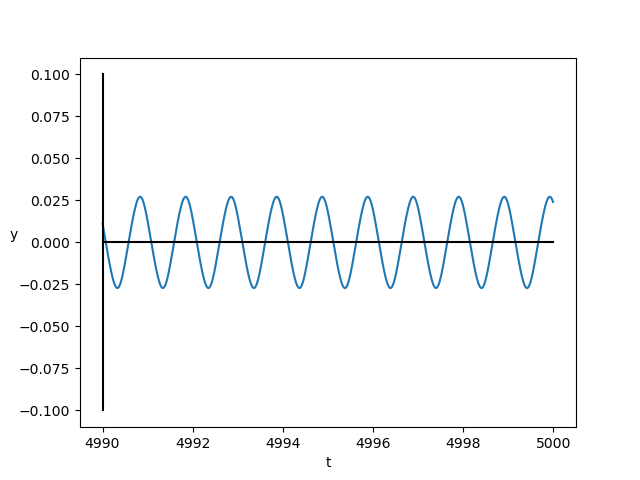
\includegraphics[scale=0.4]{plus1beta=1_005eps=0_01_4990-5000}}
\end{minipage}
\begin{minipage}[h]{0.49\linewidth}
\center{d)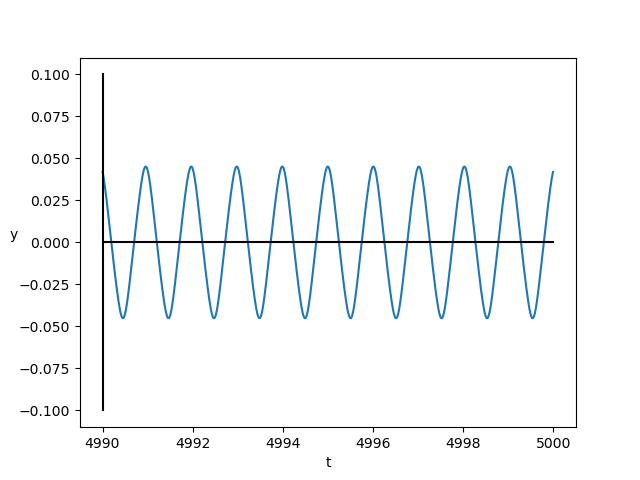
\includegraphics[scale=0.4]{plus1beta=1_01eps=0_01_4990-5000}}
\end{minipage}
\caption{Graph of the solution of the equation \eqref{f:23} at $\beta_1=1+\eps^2\beta, \;\eps=0.01, \;k=2,$a) $\beta=12.5$, b) $\beta=25$, c) $\beta=50$, d) $\beta=100$.}%picture caption
\label{fig:6}
\end{figure}

\newpage
Note that with a significant increase in the parameter $\beta$, the oscillatory mode changes, namely, the length of the period and the amplitude become larger. Numerical studies are shown in Fig. 5:
\begin{figure}[h!]
\begin{minipage}[h]{0.49\linewidth}
\center{a)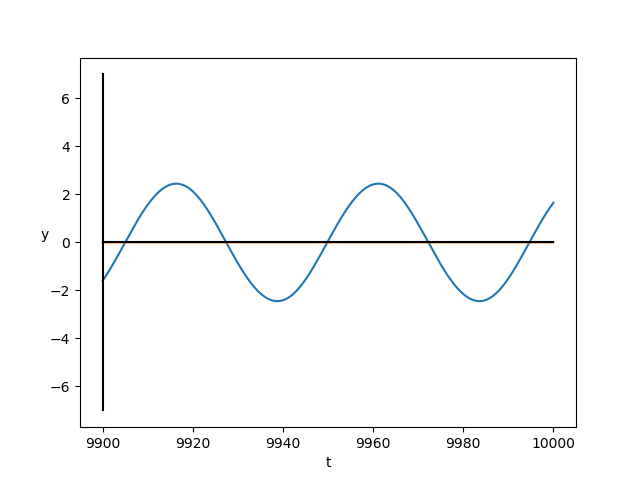
\includegraphics[scale=0.4]{plus1beta=1_02eps=0_01_9900-10000}}
\end{minipage}
\begin{minipage}[h]{0.49\linewidth}
\center{b)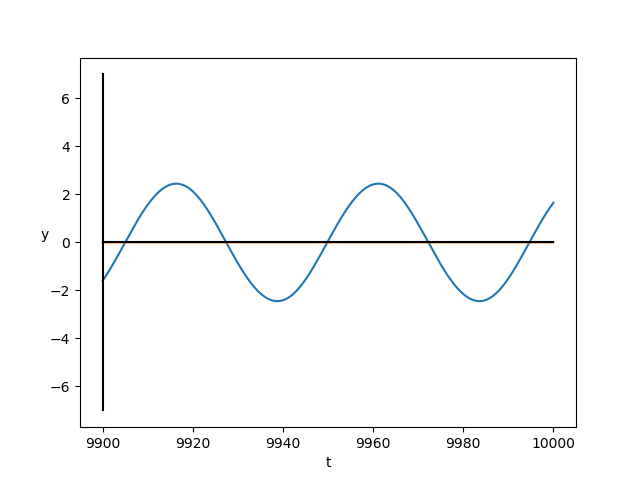
\includegraphics[scale=0.4]{plus1beta=1_025eps=0_01_9900-10000}}
\end{minipage}
\begin{minipage}[h]{0.49\linewidth}
\center{in)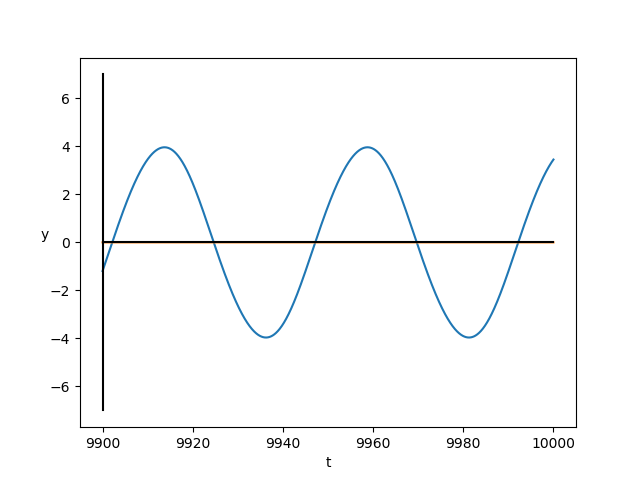
\includegraphics[scale=0.4]{plus1beta=1_05eps=0_01_9900-10000}}
\end{minipage}
\begin{minipage}[h]{0.49\linewidth}
\center{d)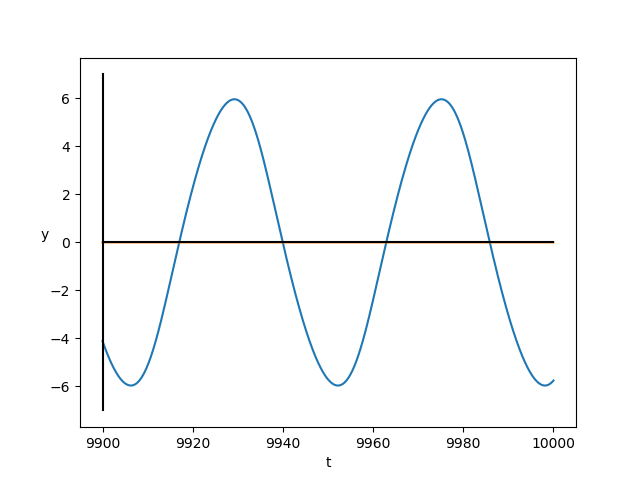
\includegraphics[scale=0.4]{plus1beta=1_1eps=0_01_9900-10000}}
\end{minipage}
\caption{Graph of the solution of the equation \eqref{f:23} at $\beta_1=1+\eps^2\beta, \;\eps=0.01,\; k=2,$a) $\beta=200$, b) $\beta=250$, c) $\beta=500$, d) $\beta=1000$.}%picture caption
\label{fig:7}
\end{figure}






\newpage
\addcontentsline{toc}{section}{Conclusion}
\section*{Conclusion}
A second-order equation with a delay in the derivative was considered, and its equilibrium state was found. To study the local dynamics of the equation, a characteristic quasi-polynomial was considered. The critical values of the parameter \(\beta_1\) are highlighted, at which the equilibrium state changes its stability. An asymptotic representation of the roots of the characteristic quasi-polynomial is found at the critical value of the parameter \(\beta_1\). It turns out to be interesting that in addition to the main infinite <<chain>> of roots tending to the imaginary axis, there is another root of the characteristic equation close to zero or a pair of such roots. An asymptotic representation of the roots is constructed with a small change in the parameter \(\beta_1\). An analogue of the normal form of the solution of the equation \eqref{f:9} with critical parameters \(\beta_1\). The corresponding numerical solutions of the initial system are presented in cases when the parameter values are close to critical.

\newpage
\addcontentsline{toc}{section}{References}
\section*{References}

\begin{enumerate}


\bibitem{S1}
{\it Larger L., Maistrenko Y., Penkovskyi B..} Virtual Chimera States for Delayed-Feedback
Systems// Physical Review Letters, 2013. Vol. 111. pp. 054103.

\bibitem{P1} 
{\it Минорский В.П.} Уравнение Минорского. // Обыкновенные дифференциально-разностные уравнения. М.: 1961. с. 191- 210 с.


\bibitem{M1}
{\it Маслеников И.Н.} Исследование локальной динамики дифференциально - интегрального уравнения с запаздыванием. // Современные проблемы математики и информатики. Выпуск 18, 2018, с. 39-45.

\bibitem{M2}
{\it Маслеников И.Н.} Локальная динамика опто-электронного осциллятора. // Современные проблемы математики и информатики. Выпуск 19, 2019, с. 44-52.

\bibitem{M3}
{\it Маслеников И.Н.} Исследование локальной динамики модели оптоэлектронного осциллятора.// Державинский форум. Тамбов, 2019, с. 157-166.



\bibitem{S2} 
Григорьева Е.В., Кащенко С.А., Глазков Д.В.. Особенности локальной динамики модели оптико-электронного осциллятора с запаздыванием. // Моделирование и анализ информационных систем. Т.25, №1, 2018, с. 71-82.

\bibitem{S3} 
Григорьева Е.В., Кащенко С.А..Нормализованные краевые задачи в модели оптико-электронного осциллятора с запаздыванием. // Прикладные задачи нелинейной теории колейбаний и волн. Известия вузов. ПНД. 2020. Т. 28, вып. 4. С. 361-382.

\bibitem{S4} 
Grigorieva E. V.,  Kashchenko S. A.. Rectangular structures in themodel of an optoelect - ronic oscillator with delay. // Physica D: Nonlinear Phenomen. 2021. 

URL:  www.elsevier.com/locate/physd 



\bibitem{K1}
{\it Кащенко И.С.} Асимптотическое разложение решений уравнений: методические указания. Ярославль: ЯрГУ, 2011.

\bibitem{K2}
{\it Кащенко И.С.} Метод квазинормальных форм в уравнениях с запаздыванием: методические указания. Ярославль: ЯрГУ, 2011.


\bibitem{Z2}
{\it Хейл Дж.} Теория функционально-дифференциальных уравнений. М.: Мир, 1984.

\end{enumerate}




\end{document}
